%% =====================================================================
%%  VL401: RTL Design and Verification -- Course Project Report
%%  P04: Ring-Oscillator PUF Key Generator with Fuzzy Extractor
%%  Built from VL401_Report_Template.tex. Every number in this report was measured
%%  in our simulations, Vivado reports or on the Zybo Z7-10 board; the sources are
%%  named in the text (files in the repository).
%% =====================================================================
\documentclass[11pt,a4paper]{article}

\usepackage[T1]{fontenc}
\usepackage[utf8]{inputenc}
\IfFileExists{lmodern.sty}{\usepackage{lmodern}}{}
\usepackage[margin=2.2cm]{geometry}
\usepackage{amsmath,amssymb}
\usepackage{graphicx}
\usepackage{booktabs,tabularx,multirow,array}
\usepackage[table]{xcolor}
\usepackage{enumitem}
\usepackage{listings}
\usepackage{caption}
\usepackage{float}
\usepackage{fancyhdr}
\usepackage{tikz}
\usetikzlibrary{arrows.meta,positioning,shapes.geometric,fit,calc}
\usepackage[colorlinks=true,linkcolor=blue!50!black,citecolor=blue!50!black,urlcolor=blue!50!black]{hyperref}

%% =====================================================================
%%  GROUP DETAILS
%% =====================================================================
\newcommand{\groupno}{XX}                         % TODO: group number
\newcommand{\projno}{P04}
\newcommand{\projtitle}{Ring-Oscillator PUF Key Generator with Fuzzy Extractor}
\newcommand{\studentA}{Student 1 Name}            % TODO: your name
\newcommand{\rollA}{B2XXXX}                       % TODO: your roll number
\newcommand{\studentB}{Arth Saxena}               % from the git history -- please confirm
\newcommand{\rollB}{B23250}                       % from the git history -- please confirm
\newcommand{\repourl}{https://github.com/MRqwertyu/Ring-Oscillator-PUF-Key-Generator}
\newcommand{\submitdate}{\today}

\newif\ifguidance
\guidancefalse

%% =====================================================================
%%  Helper macros (from the template)
%% =====================================================================
\definecolor{iitblue}{RGB}{0,51,102}
\definecolor{guidebg}{RGB}{232,240,252}
\newcommand{\guide}[1]{\ifguidance\par\noindent
  \colorbox{guidebg}{\parbox{\dimexpr\linewidth-2\fboxsep}{\small\itshape
  \textbf{Guidance:} #1}}\par\medskip\fi}

\newcommand{\figfile}[4]{%
\begin{figure}[H]\centering
\IfFileExists{#1}{\includegraphics[width=#2]{#1}}%
{\fbox{\parbox[c][4cm][c]{#2}{\centering\color{gray}\small
  [Placeholder: put \texttt{\detokenize{#1}} in this folder]}}}
\caption{#3}\label{#4}
\end{figure}}

\lstdefinelanguage{SMV}{morekeywords={MODULE,VAR,ASSIGN,DEFINE,init,next,case,esac,
  SPEC,CTLSPEC,LTLSPEC,FAIRNESS,boolean,AG,AF,AX,EG,EF,EX,A,E,U,TRUE,FALSE},
  sensitive=true,morecomment=[l]{--}}
\lstdefinelanguage{rvasm}{morekeywords={li,la,lw,sw,lbu,andi,beqz,bnez,call,ret,addi,mv,j,xor,or,srl,sll,add,sub,blt,seqz},
  sensitive=true,morecomment=[l]{\#}}
\lstset{basicstyle=\ttfamily\footnotesize,keywordstyle=\color{iitblue}\bfseries,
  commentstyle=\color{gray}\itshape,numbers=left,numberstyle=\tiny\color{gray},
  frame=single,rulecolor=\color{gray!50},breaklines=true,columns=fullflexible,
  captionpos=b,xleftmargin=1.5em,framexleftmargin=1.2em}

\setlength{\parskip}{4pt}
\setlength{\parindent}{0pt}
\setlength{\emergencystretch}{3em}
\setlist{nosep,leftmargin=1.4em}

\pagestyle{fancy}
\fancyhf{}
\lhead{\small VL401 Course Project -- Group \groupno}
\rhead{\small \projno: RO-PUF Key Generator}
\cfoot{\small \thepage}

\tikzset{blk/.style={draw,rounded corners=2pt,align=center,font=\footnotesize,minimum height=7mm,inner sep=3pt},
         arr/.style={-{Stealth[length=2mm]},thick}}

\begin{document}

%% =====================================================================
%%  TITLE PAGE
%% =====================================================================
\begin{titlepage}
\centering
{\large Indian Institute of Technology Mandi}\\[2pt]
{\normalsize School of Computing and Electrical Engineering}\\[1.6cm]
{\Large\bfseries VL401: RTL Design and Verification}\\[4pt]
{\large Course Project Report -- Odd Semester 2026}\\[1.6cm]
{\color{iitblue}\rule{\linewidth}{1pt}}\\[8pt]
{\LARGE\bfseries \projno: \projtitle}\\[8pt]
{\color{iitblue}\rule{\linewidth}{1pt}}\\[1.4cm]
{\large Group \groupno}\\[10pt]
\begin{tabular}{ll}
\toprule
\textbf{Name} & \textbf{Roll No.}\\
\midrule
\studentA & \rollA\\
\studentB & \rollB\\
\bottomrule
\end{tabular}\\[1.2cm]
\begin{tabular}{rl}
Instructor: & Dr.\ Bikram Paul\\
Repository: & \url{\repourl}\\
Submitted on: & \submitdate\\
\end{tabular}
\vfill
\begin{minipage}{0.92\linewidth}\small
\textbf{Declaration.} We declare that the RTL, verification code and analysis in this report are our own
work, except where sources (including open-source IP and AI tools) are acknowledged in
Section~\ref{sec:contrib}.\\[1.0cm]
\rule{5.5cm}{0.4pt}\hfill\rule{5.5cm}{0.4pt}\\
\studentA\hfill\studentB
\end{minipage}
\end{titlepage}

%% =====================================================================
\begin{abstract}
A physically unclonable function (PUF) derives a device-unique secret from manufacturing variation, so
a key never has to be stored. We built a complete ring-oscillator (RO) PUF key generator on a Zybo Z7-10
(Zynq-7010): 768 hand-placed configurable ROs, a code-offset fuzzy extractor (repetition-3 concatenated
with BCH(15,7,2)) whose BCH decoder was derived by hand HLS (34 cycles with one GF(2$^4$) multiplier,
18 cycles with two), a SipHash-2-4 core used as key-derivation function and MAC, a one-time enrolment
lock, and our own RV32I SoC that runs a challenge--response authentication program with the helper data
in SoC memory. Following Maiti and Schaumont's configurable RO-PUF, every RO selects one of eight LUT
paths at no extra LUT cost. On the board the baseline PUF showed 0.2--3.3\% bit-error rate (room and
+7\,$^\circ$C), while the configurable PUF showed no bit errors in 1\,800 reads; with ECC no key failed in
1\,800 reads. The design was verified against a Python golden model, 12 SystemVerilog assertions and an
explicit-state CTL model checker (seven properties hold, three injected bugs found). The SoC meets
125\,MHz, uses 52\% of the LUTs, authenticates the enrolled device and rejects the other PUF instances.
\end{abstract}

\tableofcontents
\newpage

%% =====================================================================
\section{Introduction}
\label{sec:intro}
Embedded devices need secret keys for authentication, but a key stored in flash can be read out by an
attacker with physical access. A PUF avoids storage: the key is re-created from tiny, random differences
between nominally identical circuits every time it is needed~\cite{suh07}. RO-PUFs suit FPGAs because a
ring oscillator is only a few LUTs. Their response is noisy, so a fuzzy extractor~\cite{dodis04} with
error-correcting codes is required to turn it into a stable key. An RTL implementation keeps the key
inside the hardware: software can request a MAC tag but can never read the key.

\subsection{Objectives}
\begin{enumerate}
  \item Place 128--256 ROs with Pblock/LOC constraints and build a counter-based pairwise comparator
        giving a 128-bit response.
  \item Implement a code-offset fuzzy extractor (repetition $\circ$ BCH(15,7,2)) with enrolment,
        reconstruction and a one-time enrolment lock; the key is used only internally (keyed MAC).
  \item Derive the BCH syndrome + Peterson locator by hand HLS with 1 and 2 GF(2$^4$) multipliers, and the
        GF(2$^4$) multiplier/inverse by ESPRESSO with BDD verification.
  \item Integrate everything into an RV32 SoC with a challenge--response program, helper data in SoC memory.
  \item Verify by simulation against a golden model and prove two CTL properties: the key is valid only
        after ECC success, and no enrolment is possible after the lock.
  \item Measure uniqueness, reliability (${\ge}100$ reads and a warm test) and key-failure rate before and
        after ECC, and reproduce a published RO-PUF improvement.
\end{enumerate}
All six objectives were met on the board, with one restriction: only one board was available, so
uniqueness is measured between three RO arrays in different regions of the same die
(Section~\ref{sec:discussion}). Section~\ref{sec:related} gives the background and chosen paper,
Sections~\ref{sec:spec}--\ref{sec:fpga} the design, verification and results, and
Sections~\ref{sec:discussion}--\ref{sec:conclusion} the discussion.

%% =====================================================================
\section{Background and Related Work}
\label{sec:related}

\subsection{Background}
\textbf{RO-PUF.} Suh and Devadas~\cite{suh07} compare the frequencies of RO pairs; each comparison gives
one bit. Comparing neighbours cancels effects common to both ROs (temperature, supply), leaving the
random process variation. Maiti \emph{et al.}~\cite{maiti10} characterised RO-PUFs on many FPGAs and
found close-to-ideal uniqueness but a few percent of unstable bits. \textbf{Fuzzy extractor.} Dodis
\emph{et al.}~\cite{dodis04} define the code-offset construction: at enrolment the public helper data
is $h = w \oplus c$ for a random codeword $c$; later $w' \oplus h$ is decoded to $c$ and $w = c\oplus h$
is recovered exactly. B\"osch \emph{et al.}~\cite{bosch08} showed that concatenating a repetition code
with a BCH code is an area-efficient choice on FPGAs. \textbf{BCH decoding.} For $t=2$ the error-locator
polynomial follows directly from the syndromes (Peterson~\cite{peterson60}) and its roots are found by
Chien search~\cite{chien64}; all arithmetic is in GF(2$^4$) with $p(x)=x^4+x+1$. \textbf{SipHash}~\cite{siphash}
is a 128-bit-key ARX pseudo-random function; we use it for key derivation, the key-check value and the
MAC. Yin and Qu~\cite{yin09} proposed temperature-aware cooperative RO-PUFs, an alternative way to reduce
unstable bits.

\subsection{Chosen Paper and Paper-to-RTL Plan}
\begin{table}[H]\centering\small
\caption{Paper-to-RTL contract.}\label{tab:contract}
\begin{tabularx}{\linewidth}{@{}lX@{}}
\toprule
Paper & A.~Maiti and P.~Schaumont, ``Improved ring oscillator PUF: an FPGA-friendly secure primitive,''
\emph{J.\ Cryptology}, vol.~24, no.~2, pp.~375--397, 2011, doi:10.1007/s00145-010-9088-4~\cite{maiti11}.\\
Technique & Each RO can be configured into several slightly different paths; at enrolment every pair
uses the configuration that maximises its frequency difference, stored as helper data.\\
Claim to reproduce & Fewer unstable bits (better reliability) without adding ROs, with uniqueness kept.\\
Block affected & \texttt{ro\_cell} (configuration inputs), \texttt{puf\_measure} (SELECT mode), helper data
(+384 bits), firmware (enrolment runs SELECT).\\
Baseline & The same arrays with configuration 000 (one bitstream serves both).\\
Metrics & Bit-error rate at room and warm temperature, uniqueness, bit-aliasing, key failure before and
after ECC, extra LUTs, enrolment time.\\
\bottomrule
\end{tabularx}
\end{table}

%% =====================================================================
\section{Specification and Golden Model}
\label{sec:spec}
\textbf{Specification.} 125\,MHz system clock (Zybo Z7-10 oscillator); 128-bit response from 128 RO
pairs; 128-bit key; repetition factor $r$ chosen from the measured BER for a key-failure target of
$10^{-6}$; whole SoC within the Zynq-7010 (17\,600 LUTs); no bus path to the key.

\textbf{Golden model.} A bit-exact Python model (\texttt{model/}) implements GF(2$^4$), BCH(15,7,2),
the repetition code, the code-offset fuzzy extractor and SipHash-2-4. Its 35 unit tests include an
exhaustive BCH test (all 128 codewords $\times$ 121 error patterns of weight $\le2$) and the official
SipHash vectors. \texttt{gen\_vectors.py} writes the test vectors used by every testbench: GF tables
(256+16), BCH encoder (128), BCH decoder (17\,488 with all intermediate values), SipHash (278) and
end-to-end fuzzy-extractor life cycles (24 per $r$). An analytic model gives the tolerable BER for a
$10^{-6}$ key-failure rate: 0.07\% ($r{=}1$), 1.87\% ($r{=}3$) and 5.21\% ($r{=}5$). On the Y-chart the
design starts at the behavioural level (Python algorithms), is refined to structural RTL (FSMDs and
datapaths) and is placed and routed on the physical level, where the RO placement and routing are fixed
by hand.

\begin{figure}[H]\centering
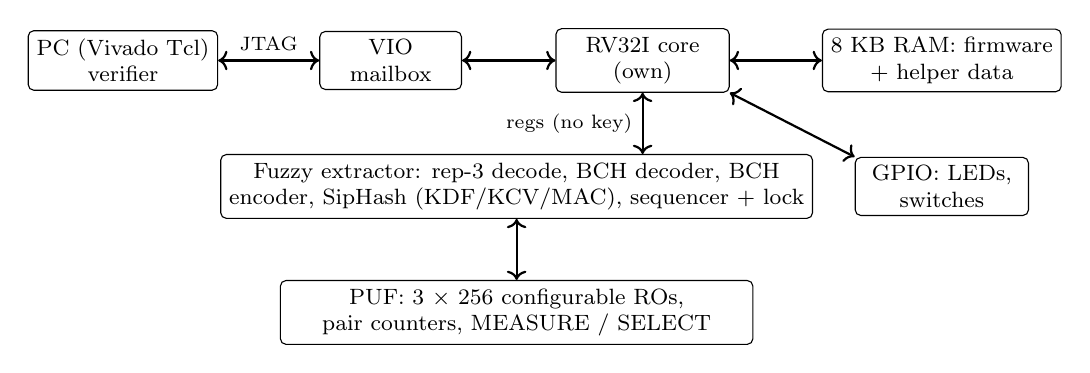
\begin{tikzpicture}
\node[blk,minimum width=24mm] (pc)   at (0,0)    {PC (Vivado Tcl)\\verifier};
\node[blk,minimum width=18mm] (vio)  at (3.4,0)  {VIO\\mailbox};
\node[blk,minimum width=22mm] (cpu)  at (6.6,0)  {RV32I core\\(own)};
\node[blk,minimum width=22mm] (ram)  at (10.4,0) {8 KB RAM: firmware\\+ helper data};
\node[blk,minimum width=22mm] (gpio) at (10.4,-1.6) {GPIO: LEDs,\\switches};
\node[blk,minimum width=60mm] (fe)   at (5.0,-1.6) {Fuzzy extractor: rep-3 decode, BCH decoder, BCH\\
encoder, SipHash (KDF/KCV/MAC), sequencer + lock};
\node[blk,minimum width=60mm] (puf)  at (5.0,-3.2) {PUF: 3 $\times$ 256 configurable ROs,\\pair counters, MEASURE / SELECT};
\draw[arr,<->] (pc) -- node[above,font=\scriptsize]{JTAG} (vio);
\draw[arr,<->] (vio) -- (cpu);
\draw[arr,<->] (cpu) -- (ram);
\draw[arr,<->] (cpu.south) -- node[left,font=\scriptsize]{regs (no key)} (cpu.south |- fe.north);
\draw[arr,<->] (fe) -- (puf);
\draw[arr,<->] (cpu.south east) -- (gpio.north west);
\end{tikzpicture}
\caption{Top-level block diagram of the key generator inside our RV32 SoC (\texttt{rtl/top/top\_soc.v}).}\label{fig:block}
\end{figure}

\begin{table}[H]\centering\small
\caption{Register map of the key generator (base 0x1000\_0000; mailbox at 0x2000\_0000, GPIO at 0x3000\_0000).}\label{tab:regmap}
\begin{tabular}{@{}llllp{5.4cm}@{}}
\toprule
Offset & Name & Access & Reset & Description\\
\midrule
0x00 & FE\_CMD & WO & -- & 1 MEASURE, 2 ENROL, 3 RECONSTRUCT, 4 LOCK, 5 MAC\\
0x04 & FE\_STATUS & RO & 0x0 & bit0 busy, 1 done, 2 cmd\_err, 3 locked, 4 key\_valid, 5 ecc\_ok, 6 kcv\_ok\\
0x08/0C & ENROL\_MSG0/1 & WO & 0x0 & random BCH messages (56 bits)\\
0x10--20 & HELPER\_IN[0..3], KCV\_IN & WO & 0x0 & helper data for RECONSTRUCT\\
0x24/28 & CHAL0/1 & WO & 0x0 & 64-bit challenge\\
0x30--48 & HELPER\_OUT, KCV\_OUT, TAG0/1 & RO & 0x0 & enrolment result, 64-bit MAC tag\\
0x50 & PUF\_CTRL & RW & 0x0 & W: bit0 start SELECT; R: bit0 busy, bit1 select done\\
0x54 & DEV\_SEL & RW & 0x0 & RO array (device) 0--2\\
0x80--AC & PAIR\_CFG[0..11] & RW & 0x0 & RO configuration of all 128 pairs (384 bits)\\
0xC0--EC & CFG\_BEST[0..11] & RO & 0x0 & result of the last SELECT\\
\bottomrule
\end{tabular}
\end{table}

%% =====================================================================
\section{High-Level Representation and Hand HLS}
\label{sec:hls}
The HLS kernel is the BCH(15,7,2) decoder (\texttt{rtl/ecc/bch\_dec\_1mul.v}, \texttt{bch\_dec\_2mul.v}).

\subsection{CDFG and Transformations}
Figure~\ref{fig:cdfg} shows the data-flow of the Peterson step before and after the key transformation,
and one Chien-search iteration. Table~\ref{tab:transform} counts the operations per decoded 15-bit word
as each transformation is applied (counts derived from the algorithm).

\begin{figure}[H]\centering
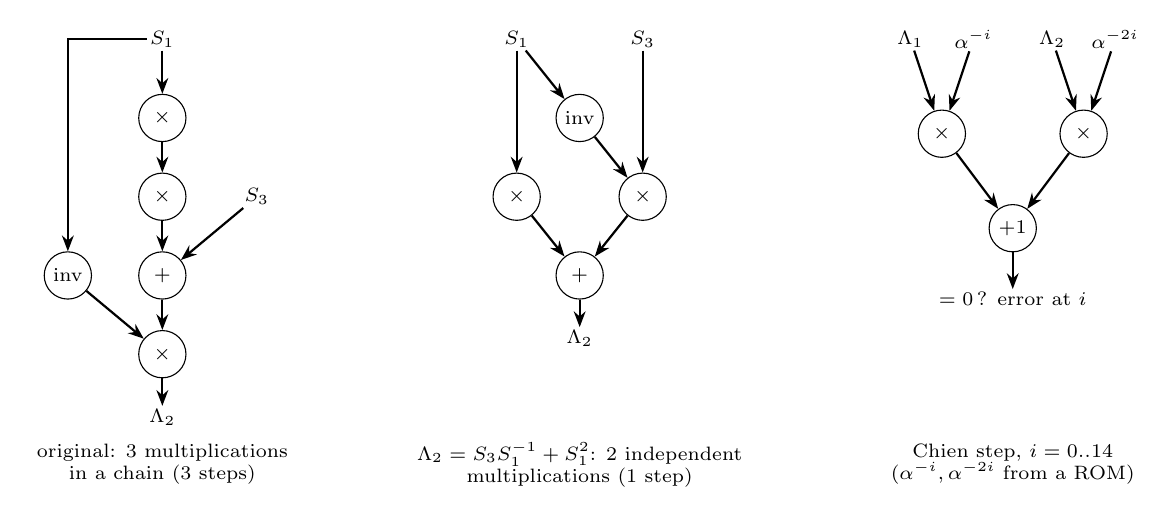
\begin{tikzpicture}[op/.style={draw,circle,inner sep=1pt,minimum size=6mm,font=\scriptsize},
                    inp/.style={font=\scriptsize,inner sep=1pt}]
% original form: S1*S1 -> *S1 -> +S3 -> *S1^-1  (three dependent multiplications)
\node[inp] (a1) at (0,0) {$S_1$};
\node[op] (m1) at (0,-1) {$\times$};
\node[op] (m2) at (0,-2) {$\times$};
\node[inp] (b1) at (1.2,-2) {$S_3$};
\node[op] (ad) at (0,-3) {$+$};
\node[op] (iv) at (-1.2,-3) {inv};
\node[op] (m3) at (0,-4) {$\times$};
\node[inp] (o1) at (0,-4.8) {$\Lambda_2$};
\draw[arr] (a1)--(m1); \draw[arr] (m1)--(m2); \draw[arr] (m2)--(ad); \draw[arr] (b1)--(ad);
\draw[arr] (ad)--(m3); \draw[arr] (iv)--(m3); \draw[arr] (m3)--(o1);
\draw[arr] (a1) -| (iv);
\node[font=\scriptsize,align=center] at (0,-5.4) {original: 3 multiplications\\in a chain (3 steps)};
% transformed form: S1*S1 and S3*S1^-1 in parallel
\begin{scope}[xshift=45mm]
\node[inp] (c1) at (0,0) {$S_1$}; \node[inp] (c3) at (1.6,0) {$S_3$};
\node[op] (iv2) at (0.8,-1) {inv};
\node[op] (ma) at (0,-2) {$\times$}; \node[op] (mb) at (1.6,-2) {$\times$};
\node[op] (ad2) at (0.8,-3) {$+$};
\node[inp] (o2) at (0.8,-3.8) {$\Lambda_2$};
\draw[arr] (c1)--(ma); \draw[arr] (c1)--(iv2); \draw[arr] (iv2)--(mb); \draw[arr] (c3)--(mb);
\draw[arr] (ma)--(ad2); \draw[arr] (mb)--(ad2); \draw[arr] (ad2)--(o2);
\node[font=\scriptsize,align=center] at (0.8,-5.4) {$\Lambda_2=S_3S_1^{-1}+S_1^2$: 2 independent\\multiplications (1 step)};
\end{scope}
% one Chien iteration
\begin{scope}[xshift=95mm]
\node[inp] (l1) at (0,0) {$\Lambda_1$}; \node[inp] (x) at (0.8,0) {$\alpha^{-i}$};
\node[inp] (l2) at (1.8,0) {$\Lambda_2$}; \node[inp] (x2) at (2.6,0) {$\alpha^{-2i}$};
\node[op] (mc) at (0.4,-1.2) {$\times$}; \node[op] (md) at (2.2,-1.2) {$\times$};
\node[op] (ev) at (1.3,-2.4) {$+1$};
\node[inp] (z) at (1.3,-3.3) {$=0$\,? error at $i$};
\draw[arr] (ev)--(z);
\draw[arr] (l1)--(mc); \draw[arr] (x)--(mc); \draw[arr] (l2)--(md); \draw[arr] (x2)--(md);
\draw[arr] (mc)--(ev); \draw[arr] (md)--(ev);
\node[font=\scriptsize,align=center] at (1.3,-5.4) {Chien step, $i=0..14$\\($\alpha^{-i},\alpha^{-2i}$ from a ROM)};
\end{scope}
\end{tikzpicture}
\caption{Data-flow graphs: Peterson step before (left) and after (middle) the algebraic transformation; one Chien iteration (right).}\label{fig:cdfg}
\end{figure}

\begin{table}[H]\centering\small
\caption{Effect of the transformations (per decoded word; ``const.'' = multiplication by a constant power of $\alpha$).}\label{tab:transform}
\begin{tabularx}{\linewidth}{@{}Xcccc@{}}
\toprule
Version & \#Mult & \#Mult & \#Add & Peterson crit.\\
 & (general) & (const.) & (XOR) & path (steps)\\
\midrule
Textbook: Horner syndromes $S_1..S_4$, $\Lambda_2=(S_3+S_1^3)/S_1$, Chien squares $x$ & 48 & 56 & 87 & 3\\
+ redundancy removal: $S_2=S_1^2$, $S_4=S_1^4$ not computed & 48 & 28 & 59 & 3\\
+ syndromes as constant XOR networks (precomputed $\alpha^{i}$, $\alpha^{3i}$) & 48 & 0 & 59 & 3\\
+ strength reduction: $\alpha^{-2i}$ read from a ROM instead of squaring & 33 & 0 & 59 & 3\\
+ tree-height reduction: $\Lambda_2 = S_3S_1^{-1}+S_1^2$ & \textbf{32} & \textbf{0} & \textbf{59} & \textbf{1}\\
\bottomrule
\end{tabularx}
\end{table}

\subsection{Operator Library}
Characterised by out-of-context synthesis on the Zynq-7010 (scripts \texttt{synth\_gf.tcl} and
\texttt{synth\_bch.tcl}): GF(2$^4$) multiplier, ESPRESSO SOP form 16 LUTs / 3.31\,ns, XOR (Mastrovito~\cite{mastrovito88}) form
8 LUTs / 3.17\,ns; inverse 4 LUTs / 2.07\,ns; 4-bit GF addition one LUT level; syndrome XOR network
12 LUTs; Chien constant ROM 3 LUTs. An inverse, a multiplication and an addition fit in one 8\,ns
step, so the inverse and the XORs are \emph{chained} with the multiplier and each multiplication takes
one control step.

\subsection{Scheduling}
With unit-time multiplications the two Peterson products are independent: ASAP puts both in the first
Peterson step and, with a two-step bound, ALAP in the second, so each has mobility 1. The same holds for
the two products of every Chien position, which start after $\Lambda_1,\Lambda_2$ are known; no
multiplication depends on another one of the same kernel. List scheduling (priority = least mobility, then program
order) gives: \textbf{2 multipliers} -- Peterson 1 step, Chien 15 steps; \textbf{1 multiplier} -- Peterson
2 steps ($S_1^2$, then $S_3S_1^{-1}$), Chien 30 steps. With syndromes and the final check this is
\textbf{18} and \textbf{34} cycles. Both schedules meet the resource lower bound
$\lceil 32/\#\text{mult}\rceil$ multiplier steps (16 and 32), so they are optimal; we therefore did not
run FDS or ILP.

\subsection{Allocation and Binding}
\textbf{FU binding.} Two multiplications are compatible when they are in different steps. In the
2-multiplier schedule each step holds two multiplications, so the compatibility graph partitions into
exactly two cliques: MA = $\{S_1\!\cdot\!S_1,\ \Lambda_1\alpha^{-i}\}$ and MB = $\{S_3\!\cdot\!S_1^{-1},\
\Lambda_2\alpha^{-2i}\}$; with one multiplier all 32 multiplications form one clique, at the price of a
4-way operand multiplexer. \textbf{Register binding} (left-edge over the value lifetimes): $r$ (whole
decode), $S_1,S_3$ and $\Lambda_1,\Lambda_2$ (until the check; they are also outputs), position $i$,
root counter and error mask. In the 1-multiplier design $\Lambda_2$ doubles as the accumulator between
the two Peterson steps, and one extra register (\texttt{acc}, 4 bits) plus a \texttt{phase} bit holds
$1+\Lambda_1\alpha^{-i}$ between the two Chien sub-steps: exactly the 5 extra flip-flops seen in
Table~\ref{tab:designpoints}.

\subsection{FSMD and Design Points}
Each control step became one FSM state (IDLE, SYN, P1[,P2], CHIEN, CHECK) driving the operand
multiplexers and register enables. The decoder is constant-time (latency independent of the error
pattern). Both design points were implemented and verified on all 17\,488 vectors (Section~\ref{sec:sim}).

\begin{table}[H]\centering\small
\caption{Design points (Zynq-7010, out of context, hierarchy kept, ESPRESSO multiplier; \texttt{docs/reports/synth\_bch/}).}\label{tab:designpoints}
\begin{tabular}{@{}lcccccc@{}}
\toprule
Design point & LUT & FF & DSP & F$_\text{max}$ (MHz) & Latency (cycles) & Latency (ns)\\
\midrule
Min-latency: 2 multipliers & 125 & 57 & 0 & 161.8 & 18 & 111.2\\
Min-area: 1 multiplier     & 110 & 62 & 0 & 158.5 & 34 & 214.5\\
\bottomrule
\end{tabular}
\end{table}
With the XOR multiplier the two points are 107 and 101 LUTs. The 2-multiplier design has a 41\% better
area--latency product: a 16-LUT multiplier is too small for sharing to pay for its multiplexers. With
Vivado's default flattening the 1-multiplier ESPRESSO design grew to 243 LUTs, because the 129-term SOP
was merged with its operand multiplexer.

%% =====================================================================
\section{Logic and FSM Optimisation}
\label{sec:logic}

\subsection{State Minimisation}
The key-generator sequencer (\texttt{rtl/fe/fuzzy\_extractor.v}) has 12 states. In the implication-chart
analysis every pair of states is distinguished in the first step: IDLE, MEAS\_REQ (\texttt{puf\_req}),
ENC (helper write), REPDEC (vote register load), BCH\_START (\texttt{dec\_start}), REBUILD (response
rebuild), H\_INIT (\texttt{sip\_init}), H\_BLK (\texttt{sip\_valid}) and FINISH (\texttt{done}) each assert
a different control output, and the three wait states (MEAS\_WAIT, BCH\_WAIT, H\_WAIT) react to different
inputs (\texttt{puf\_valid}, \texttt{dec\_done}, \texttt{tag\_valid}) with different successors. No pair is
equivalent, so the FSM is already minimal.

\subsection{State Encoding}
\begin{table}[H]\centering\small
\caption{State encodings of the whole fuzzy extractor ($r=3$), Vivado \texttt{-fsm\_extraction}; 125\,MHz constraint, post-synthesis (\texttt{scripts/synth\_fsm\_encoding.tcl}).}\label{tab:encoding}
\begin{tabular}{@{}lcccc@{}}
\toprule
Encoding & Sequencer state bits & LUT & FF & F$_\text{max}$ (MHz)\\
\midrule
Binary (as written in the RTL) & 4 & 1346 & 1142 & 138.6\\
One-hot$^{*}$ & 4 & 1520 & 1142 & 138.6\\
Sequential & 4 & 1320 & 1138 & 138.6\\
Gray & 4 & 1327 & 1139 & 138.6\\
Johnson & 6 & 1397 & 1140 & 138.6\\
\bottomrule
\end{tabular}
\end{table}
$^{*}$Vivado re-encoded all three FSMs (sequencer, BCH decoder, SipHash), except that in the one-hot run
it kept the sequencer binary and one-hot-encoded only the BCH and SipHash FSMs. F$_\text{max}$ does not change because the critical path is a SipHash round,
not the controllers. Sequential and Gray are the smallest (1.9\% and 1.4\% below binary); one-hot, applied to the BCH and
SipHash FSMs, costs 13\% more LUTs; Johnson costs 4\% more.

\subsection{Two-Level Minimisation}
The GF(2$^4$) multiplier (8 inputs, 4 outputs, 225 ON-set rows) and inverse (4 inputs, 15 ON-set rows)
were minimised with ESPRESSO~\cite{brayton84} and with our own Quine--McCluskey implementation
(\texttt{model/qm.py}: prime generation, then an exact unate-covering solver with essential primes,
row/column dominance and branch and bound).

\begin{table}[H]\centering\small
\caption{Two-level results: product terms / literals.}\label{tab:twolevel}
\begin{tabular}{@{}lcc@{}}
\toprule
Method & Multiplier & Inverse\\
\midrule
ESPRESSO heuristic, multi-output & 135 / 810 & 15 / 51\\
ESPRESSO exact (\texttt{-Dexact}), multi-output & \textbf{129 / 781} & \textbf{14 / 50}\\
Our QM + exact UCP, each output separately & 160 / 894 & 21 / 67\\
ESPRESSO exact, each output separately & 160 / 894 & 21 / 67\\
\bottomrule
\end{tabular}
\end{table}
Our QM gives exactly the same minimum as ESPRESSO for each of the eight single outputs (e.g.\ 40 terms
for every multiplier output, 45--60 primes each), which validates both. The remaining gap is product-term
sharing between outputs, which only the multi-output minimiser exploits. The ESPRESSO cover was proven
equivalent to the reference with ROBDDs (Section~\ref{sec:formal}) and simulated exhaustively.

\subsection{Multilevel Optimisation}
We did not run kernel extraction or Yosys+ABC (not installed). As the multilevel alternative we wrote
the XOR-factored Mastrovito multiplier~\cite{mastrovito88}: 16 AND2 gates form the partial products
$c_0..c_6$ and 15 XOR2 gates combine and reduce them ($p_0=c_0\oplus c_4$, $p_1=c_1\oplus c_4\oplus
c_5$, $p_2=c_2\oplus c_5\oplus c_6$, $p_3=c_3\oplus c_6$). After Vivado synthesis it needs 8 LUTs
against 16 for the 781-literal SOP: XOR-heavy functions suit multi-level logic and 6-input LUTs, not
two-level AND--OR.

%% =====================================================================
\section{RTL Design and SoC Integration}
\label{sec:rtl}

\subsection{Module Hierarchy}
\texttt{top\_soc} contains \texttt{u\_puf} (\texttt{puf\_measure} with three \texttt{ro\_array}s of 256
\texttt{ro\_cell}s), \texttt{u\_soc} (\texttt{rv32\_core}, \texttt{soc\_ram}, \texttt{fuzzy\_extractor}
with \texttt{bch\_dec\_2mul}, \texttt{bch\_enc}, \texttt{rep\_encode/decode}, \texttt{siphash24}) and
\texttt{u\_vio}. One 125\,MHz clock domain plus one domain per measured RO (counters are read only after
the gate closes and the ROs stop, so no synchroniser is needed); synchronous active-high reset;
valid/ready handshakes (PUF \texttt{puf\_req}/\texttt{puf\_valid}, CPU bus \texttt{mem\_valid}/\texttt{mem\_ready}).
\texttt{fuzzy\_extractor} has no key port; the key and response registers are wiped at the end of every
command. \textbf{Lint:} Vivado's RTL linter (\texttt{synth\_design -lint}) on all SoC RTL reported 0
errors and 5 messages, all intentional: the lock register's reset value comes from the boot-lock fuse
input; a mixed signed/unsigned add in the majority counter (value $\le5$); an unused characterisation
port; and unused address/data bits of the word-aligned RAM and load shifter.

\subsection{Bus Integration, Interrupt and DMA}
The key generator, mailbox and GPIO are memory-mapped on our own valid/ready bus (one wait state).
There is no interrupt or DMA: the firmware polls \texttt{FE\_STATUS.done}, which is enough because the
CPU has nothing else to do while a command runs. The firmware is RV32I assembly (no RISC-V compiler
ships with Vivado), assembled by our two-pass assembler \texttt{sw/rvasm.py}; the image is 904 bytes.

\begin{lstlisting}[language=rvasm,caption={Driver excerpt (\texttt{sw/firmware.S}): issue a key-generator command and wait.},label={lst:driver}]
.equ FE, 0x10000000             # key generator base
fe_cmd:                         # a0 = command (2 ENROL, 3 RECONSTRUCT, 5 MAC ...)
        sw   a0, 0x00(s0)       # FE_CMD   (s0 = FE)
fc_w:   lw   a0, 0x04(s0)       # FE_STATUS
        andi t0, a0, 2          # done?
        beqz t0, fc_w
        ret                     # a0 = status: key_valid, locked, cmd_err ...
\end{lstlisting}

\subsection{Hardware/Software Comparison}
The same BCH decode (syndromes, Peterson, Chien search; GF multiplication by log/antilog tables) was
written in RV32I software (\texttt{sw/tests/bch\_sw.S}) and run on our core in simulation on 64 words
from the golden vectors (0 mismatches). It takes \textbf{4\,542 cycles per decode} (852 instructions; our
multi-cycle core has a CPI of about 5.3), against \textbf{18 cycles} for the 2-multiplier decoder and
34 for the 1-multiplier one: a speed-up of about \textbf{252$\times$} (134$\times$). The timed software
loop includes about 10 instructions per word for checking the result, roughly 1\% of the total. At
system level the speed-up matters less: one PUF measurement takes about 8.5\,ms, while the whole
logic part of a reconstruction ($r=3$) takes about 87 cycles in simulation (0.7\,$\mu$s).

%% =====================================================================
\section{Simulation-Based Verification}
\label{sec:sim}
Every testbench is self-checking against golden-model vectors (\texttt{model/vectors/}). Directed tests
cover each block exhaustively where possible (GF tables, BCH encoder, all error patterns of weight $\le2$);
random tests use the model's random keys, messages and noise; system tests replay complete life cycles.
The fuzzy-extractor testbench additionally checks a corrupted key-check value and the boot lock. Twelve
SystemVerilog assertions are bound into \texttt{fuzzy\_extractor} (\texttt{tb/fe\_sva.sv}), e.g.\ Listing~\ref{lst:sva}:
the key is valid only with \texttt{ecc\_ok} and \texttt{kcv\_ok}; the lock is sticky; no enrolment starts
while locked; a locked ENROL is answered with \texttt{done}+\texttt{cmd\_err}; the MAC runs only with a
valid key; the key register is zero when idle without a valid key; the response register is wiped after
every command; the raw-response port stays zero; \texttt{done} and \texttt{puf\_req} are single pulses;
every command finishes within 400 cycles; \texttt{key\_valid} only rises at the end of a command.
To show that they are active, the lock-check mutant was run with them: \texttt{a\_no\_enrol} and
\texttt{a\_enrol\_reject} fired 25 times each.

\begin{lstlisting}[language=Verilog,caption={Two of the 12 assertions (\texttt{tb/fe\_sva.sv}).},label={lst:sva}]
a_key_ecc:  assert property (@(posedge clk) disable iff (rst) key_valid |-> ecc_ok && kcv_ok);
a_no_enrol: assert property (@(posedge clk) disable iff (rst)
                             !(state == S_MEAS_REQ && op == OP_ENROL && locked));
\end{lstlisting}

\begin{table}[H]\centering\small
\caption{Verification summary (Vivado xsim 2024.2).}\label{tab:simsummary}
\begin{tabular}{@{}lc@{}}
\toprule
Item & Result\\
\midrule
GF(2$^4$) multiplier / inverse (exhaustive) & 256/256, 16/16\\
BCH decoder, 4 configurations $\times$ 17\,488 vectors (all intermediate values) & 0 mismatches\\
SipHash-2-4 (64 reference + 200 random + 14 design messages) & 278/278\\
Fuzzy extractor, $r=1,3,5$: 24 life cycles each, bit-exact with the model & 72/72\\
CPU self-test program (all RV32I instruction classes) / SoC system scenario & pass / pass\\
Assertions & 12, 0 failures ($r=1,3,5$)\\
Coverage of \texttt{fuzzy\_extractor} (statement / branch / condition) & 95.4\% / 88.6\% / 100\%\\
Coverage of \texttt{siphash24} / \texttt{bch\_dec\_2mul} (statement / branch) & 98.0 / 92.3\%, 97.9 / 92.9\%\\
Mutants caught (BCH $\Lambda_2$, SipHash rotation, lock check, KCV check) & 4/4\\
\bottomrule
\end{tabular}
\end{table}
The overall statement/branch/condition coverage of the $r=3$ run including the testbench is
96.2/81.0/88.6\%; xsim reported 0.6\% toggle coverage, which we did not investigate and do not use.
The assertion counters show the corner cases were exercised: 20 valid keys, 25 refused enrolments and
4 BCH failures per run (for $r=5$ only one of the four foreign responses failed in BCH; the other three
mis-corrected and were rejected by the key-check value). \textbf{Bugs found by simulation:} the CPU's
arithmetic shift became logical (in Verilog a \texttt{?:} with an unsigned branch makes \texttt{>>>}
unsigned); the firmware lost a command sent during boot (fixed with a boot handshake); a golden-model
test case never reached BCH for $r>1$; and the KCV mutant passed all model vectors, so a dedicated
wrong-KCV test was added.

%% =====================================================================
\section{Formal Verification}
\label{sec:formal}
NuSMV and SymbiYosys were not available on the lab PC, so we wrote an explicit-state CTL model checker
(\texttt{model/ctl.py}): reachable states by BFS, EX, E[$\,$U$\,$] (least fixpoint) and EG (greatest
fixpoint) with the standard labelling algorithm~\cite{clarke86}, the other operators derived, and
shortest counterexample paths. Its unit tests check every operator on a structure with known answers.

\subsection{Kripke Structure and CTL Labelling}
Abstracting the sequencer to the lock behaviour gives four states: $s_0$ idle/unlocked, $s_1$
enrolling, $s_2$ idle/locked, $s_3$ busy/locked (reconstruct or MAC), with transitions
$s_0{\to}\{s_0,s_1,s_2\}$, $s_1{\to}s_2$ (enrolment ends with AUTO\_LOCK), $s_2{\to}\{s_2,s_3\}$,
$s_3{\to}s_2$; $locked$ holds in $\{s_2,s_3\}$, $enrol$ in $\{s_1\}$. By hand:
$\mathbf{EF}\,enrol$ = backward closure of $\{s_1\}$ = $\{s_0,s_1\}$, so $\mathbf{AG}\neg enrol$ =
$\{s_2,s_3\}$ and $locked\rightarrow\mathbf{AG}\neg enrol$ holds in every state. $\mathbf{AX}\,locked$
= $\{s_1,s_2,s_3\}$ ($s_0$ can stay unlocked), so $locked\rightarrow\mathbf{AX}\,locked$ also holds
everywhere. Adding the edge $s_2{\to}s_1$ (lock check removed) puts $s_2$ into $\mathbf{EF}\,enrol$ and
breaks the first property, which is what the full model reports below.

\subsection{Model Checking}
The full model (\texttt{model/fe\_fsm\_model.py}) follows the RTL state by state with state, operation,
SipHash job, BCH block index and the four status flags; command arrival, PUF timing, BCH success,
SipHash progress and the KCV comparison are free inputs, and the lock may start set (boot fuse). It has
238 reachable states and 448 transitions.

\begin{table}[H]\centering\small
\caption{CTL properties checked with our model checker.}\label{tab:ctl}
\begin{tabularx}{\linewidth}{@{}clXl@{}}
\toprule
\# & Type & CTL formula & Result\\
\midrule
1 & Safety (spec) & $\mathbf{AG}(\mathit{key\_valid}\rightarrow \mathit{ecc\_ok})$ & true\\
2 & Safety (spec) & $\mathbf{AG}(\mathit{locked}\rightarrow\mathbf{AG}\,\neg\mathit{enrol\_started})$ & true\\
3 & Safety & $\mathbf{AG}(\mathit{locked}\rightarrow\mathbf{AX}\,\mathit{locked})$ & true\\
4 & Safety & $\mathbf{AG}(\mathit{key\_valid}\rightarrow \mathit{kcv\_ok})$ & true\\
5 & Safety & $\mathbf{AG}(\mathit{mac\_running}\rightarrow \mathit{key\_valid})$ & true\\
6 & Safety & $\mathbf{AG}((\mathit{idle}\wedge\neg\mathit{key\_valid})\rightarrow\neg\mathit{key\_set})$ & true\\
7 & Non-blocking & $\mathbf{AG}(\mathit{busy}\rightarrow\mathbf{EF}\,\mathit{idle})$ & true\\
8 & Liveness (no fairness) & $\mathbf{AG}(\mathit{busy}\rightarrow\mathbf{AF}\,\mathit{idle})$ & false\\
9 & Reachability & $\mathbf{EF}\,\mathit{key\_valid}$; $\mathbf{EF}(\mathit{locked}\wedge\mathbf{EF}\,\mathit{key\_valid})$ & true\\
10 & Reachability & $\mathbf{EF}\,\mathit{enrol\_started}$ & true$^{a}$\\
\bottomrule
\end{tabularx}
\end{table}
$^{a}$From the unlocked initial state; false from the boot-locked one, as intended.
Property 8 fails because the PUF may never answer (MEAS\_WAIT self-loop); our checker has no fairness
constraints, so non-blocking (property 7) is the strongest progress property we prove. Property 10 shows
that the boot fuse really blocks enrolment.

\subsection{Bug Injection and Counterexamples}
Three mutants of the model were checked. \emph{Lock check removed}: property 2 fails with the
counterexample IDLE(locked) $\rightarrow$ MEAS\_REQ(ENROL). \emph{KCV result ignored}: property 4 fails
after 18 steps (all BCH blocks decode, the KCV mismatches, yet \texttt{key\_valid}=1).
\emph{BCH failure ignored}: property 1 fails after 16 steps (BCH\_WAIT $\rightarrow$ REBUILD with
\texttt{ecc\_ok}=0). The first two were also replayed in simulation: the lock mutant is caught by the
testbench and by two assertions, the KCV mutant by the wrong-KCV test. \textbf{Link to the RTL:} the
fuzzy-extractor testbench (\texttt{-d FSM\_TRACE}) writes the RTL values of all model variables every
cycle; all 3\,527 simulated cycles (76 distinct transitions) are transitions of the model.

\subsection{BDD Analysis}
With our ROBDD package (\texttt{model/bdd.py}~\cite{bryant86}) we built the GF(2$^4$) multiplier from the
truth table, from the ESPRESSO cover and from the Mastrovito equations: for every output all three give
the same node, which proves them equivalent. Shared node counts for orderings: $a_3..a_0\,b_3..b_0$
(separated) 82, interleaved MSB-first 104, interleaved LSB-first 130. Instead of sifting we evaluated
\emph{all} 40\,320 orders: minimum 82 (reached by exactly the 1\,152 orders that put all bits of one
operand first: once $a$ is fixed, the product is linear in $b$), median 106, maximum 138. Reachability
was computed explicitly (238 states), not symbolically.

\subsection{Formal Verification of the RTL (SymbiYosys)}
Not performed: SymbiYosys is not installed. The RTL-level checks are the 12 assertions in simulation
(Section~\ref{sec:sim}) and the trace-conformance check above, which ties the proven model to the RTL.

%% =====================================================================
\section{Incorporating the Research Paper}
\label{sec:paper}
Each LUT stage of \texttt{ro\_cell} receives the same signal on two physical pins (A2 and A5) and a
configuration bit selects which one is used, giving $2^3=8$ paths per RO \emph{in the same LUTs}.
\texttt{puf\_measure} gained a SELECT mode that measures all eight configurations of every pair and keeps
the one with the largest count difference; the 384-bit choice is stored as helper data in SoC RAM and
reloaded before every reconstruction. Baseline and enhanced PUF are the same bitstream (baseline =
configuration 000), measured on the same arrays, clock (125\,MHz) and protocol: 100 reads at room
temperature and 100 with the on-chip heater (die 42.5\,$\rightarrow$\,49.5\,$^\circ$C, XADC).

\begin{table}[H]\centering\small
\caption{Baseline vs.\ paper-enhanced PUF on the Zybo Z7-10 (three arrays; three builds for uniqueness).}\label{tab:paper}
\begin{tabular}{@{}lccc@{}}
\toprule
Metric & Baseline & Enhanced & Change\\
\midrule
LUT for the 768 ROs & 3\,072 & 3\,072 & 0\\
Clock (same bitstream) & 125\,MHz & 125\,MHz & --\\
Bit-error rate, room (per array, final build) & 0.67--1.86\% & 0.00\% & all errors removed\\
Bit-error rate, warm (+7\,$^\circ$C) & 0.17--3.30\% & 0.00\% & all errors removed\\
Reads with any bit error (key failure before ECC) & 78--100\% & 0\% & \\
Uniqueness, pooled over 9 array pairs & 48.9\% & 50.2\% & closer to 50\%\\
Bit-aliasing (mean over bits) & 0.52--0.55 & 0.50--0.53 & closer to 0.5\\
Helper data & 160 bits & 544 bits & +384\\
Enrolment time (measurement + SELECT) & 8.5\,ms & 76\,ms & $\times 9$\\
\bottomrule
\end{tabular}
\end{table}
BER is measured against the majority vote of the room reads. The enhancement removed every bit error we
observed (1\,800 reads over three builds), consistent with the paper's claim of a strong reliability
improvement; we did not reproduce the paper's own experimental setup, so we compare only the direction
of the effect, not its numbers. The reason is visible in Figure~\ref{fig:flip}: every unstable bit came
from a pair whose frequencies differ by less than 0.13\%, and SELECT avoids exactly these near-ties. Its
cost is no LUTs in the RO array, larger helper data and a longer enrolment. Uniqueness is measured
between die regions, not chips (Section~\ref{sec:discussion}).

\figfile{figures/hw_flip_vs_gap.png}{0.62\linewidth}{Measured flip rate of each response bit over 100 reads against the frequency gap of its RO pair (baseline).}{fig:flip}

%% =====================================================================
\section{FPGA Implementation and Demonstration}
\label{sec:fpga}
All 768 ROs are fixed with LOC, BEL and LOCK\_PINS in an exclusive Pblock (generated by
\texttt{scripts/gen\_puf\_xdc.py}). We found that a rebuild still changed 17--21\% of the response
bits, because the router re-wires each RO loop (one RO moved by 20.6\%). We therefore lock the routes of
all 2\,304 RO-internal nets with FIXED\_ROUTE, exported from the reference SoC build and verified in
every build (2\,304/2\,304 identical). A rebuild with locked routes still changed 7--10\% of the bits
(per-RO change 0.2\%, caused by the changed surroundings), so a PUF instance is tied to its bitstream and
firmware must be updated with \texttt{updatemem}, not by rebuilding.

\begin{table}[H]\centering\small
\caption{Post-implementation results of the SoC on the Zybo Z7-10 (\texttt{xc7z010clg400-1}).}\label{tab:fpga}
\begin{tabular}{@{}lc@{}}
\toprule
Item & Value\\
\midrule
Target clock & 125\,MHz\\
WNS / TNS / WHS & +0.055\,ns / 0.000\,ns / +0.038\,ns\\
LUT / FF / DSP / BRAM (whole SoC) & 9\,156 (52\%) / 9\,365 / 0 / 2\\
\quad LUT: PUF / CPU / fuzzy extr.\ / VIO+debug & 4\,953 / 1\,751 / 1\,332 / 1\,071\\
Estimated power (Vivado, vectorless) & 0.210\,W (0.119\,W dynamic)\\
\bottomrule
\end{tabular}
\end{table}
Timing closure needed two fixes: the SipHash rounds were made register-to-register after the integrated
key generator missed 125\,MHz by 0.54\,ns, and the CPU's operand-select and subtract controls were
registered one state earlier after the SoC missed by 0.019\,ns. We did not use an ILA (the SoC is
observed through the VIO mailbox); the demonstration (\texttt{scripts/hw/soc\_demo.tcl},
Listing~\ref{lst:demo}) programs the board over JTAG, enrols device 0 (a second enrolment is refused),
records eight challenge--response pairs, resets the SoC, restores the helper data, authenticates device 0
with four unused challenges, rejects devices 1 and 2 with the same helper data, and repeats the
reconstruction 100 times. It passed in both baseline and configurable mode (100/100 valid keys and
correct tags each). The characterisation results are in Figure~\ref{fig:hd}.

\begin{lstlisting}[numbers=none,caption={Excerpt of the demo log on the board (\texttt{data/hw\_soc/demo\_base.txt}, baseline mode; lines shortened).},label={lst:demo}]
ENROL device 0: key_valid=0 locked=1 cmd_err=0 ecc_ok=0 kcv_ok=0
ENROL again: ... cmd_err=1 -> REFUSED (locked)
RECONSTRUCT device 0 with restored helper data: key_valid=1 ... ecc_ok=1 kcv_ok=1
AUTH device 0: 4/4 unused challenges answered correctly -> AUTHENTICATED
IMPOSTOR device 1: reconstruct key_valid=0 ...; AUTH REJECTED
IMPOSTOR device 2: reconstruct key_valid=0 ...; AUTH REJECTED
RELIABILITY: 100/100 reconstructions gave a valid key, 100/100 answered correctly
\end{lstlisting}

\figfile{figures/hw_hd.png}{0.9\linewidth}{Measured intra-device (100 room + 100 warm reads per array) and inter-array Hamming distances.}{fig:hd}

%% =====================================================================
\section{Discussion and Limitations}
\label{sec:discussion}
The fuzzy extractor worked as designed: the measured worst-case BER (3.3\%) is above what BCH alone
tolerates (key failures up to 7\% with $r=1$ when replayed in the model) but well within repetition-3
(0 failures in 1\,800 reads; predicted $3.7\times10^{-5}$). The configurable RO was the most effective
change. \textbf{Limitations.} (i) Only one board: uniqueness is measured between three regions of one
die, not between chips. (ii) The one-time lock survives a reset only through an emulated fuse (switch
SW3); we did not burn the Zynq eFUSEs. (iii) The enrolment randomness (BCH messages) comes from the host,
not from an on-chip TRNG. (iv) With $r=3$ the response leaves at most about 14 bits of entropy after the
helper data (ideal case); a configurable-only build with $r=1$ would keep about 56 bits. (v) The PUF is
tied to its bitstream. (vi) The warm test covered only +7\,$^\circ$C. (vii) Liveness was not proven
(no fairness), and no SymbiYosys or NuSMV run was possible. With hindsight we would lock the RO routes
from the very first build and enrol from a majority vote of several reads (one noisy enrolment read
raised array 1's apparent BER from 0.72\% to 2.40\%).

%% =====================================================================
\section{Conclusion and Future Work}
\label{sec:conclusion}
The key generator runs at 125\,MHz in 52\% of a Zynq-7010, reconstructs the key in 87 logic cycles after
an 8.5\,ms PUF measurement, decodes BCH 252$\times$ faster than software on the same core, and
authenticated the enrolled device and rejected the others in every demo run. The configurable RO removed
all observed bit errors (baseline 0.2--3.3\%) at no LUT cost, and the two required CTL properties hold.
Future work: measure several boards with the same bitstream, and add an on-chip TRNG and majority-vote
enrolment.

%% =====================================================================
\section*{Contribution Statement and Acknowledgements}
\addcontentsline{toc}{section}{Contribution Statement and Acknowledgements}
\label{sec:contrib}
\begin{table}[H]\centering\small
\begin{tabularx}{\linewidth}{@{}lX@{}}
\toprule
Member & Main contributions\\
\midrule
\studentA & Golden model, ESPRESSO/BDD, hand-HLS BCH decoder, SipHash, fuzzy extractor and lock, RO-PUF
hardware and placement, characterisation, RV32 core/SoC/firmware, CTL model checking, FPGA bring-up and
demo, report.\\
\studentB & Repository set-up and an early 16-RO bank prototype (\texttt{RO/}); could not continue the
FPGA work, which was then completed by \studentA.\\
\bottomrule
\end{tabularx}
\end{table}

\textbf{Open-source IP and tools used:} Xilinx VIO and debug-hub IP (Vivado); ESPRESSO (UC Berkeley,
\texttt{classabbyamp/espresso-logic}, with our Windows patch); Python with NumPy and Matplotlib. The RISC-V
core, assembler, BDD package, QM minimiser and CTL model checker are our own.\\
\textbf{AI-tool use:} an AI coding assistant (Anthropic Claude, via Claude Code) was used throughout the
project to draft and debug RTL, testbenches, scripts and documentation, under our direction. All results
in this report come from our simulations, Vivado reports and board measurements.

%% =====================================================================
\begin{thebibliography}{99}
\bibitem{suh07} G.~E.~Suh and S.~Devadas, ``Physical unclonable functions for device authentication and
  secret key generation,'' in \emph{Proc.\ 44th Design Automation Conf.}, 2007, pp.~9--14, doi: 10.1145/1278480.1278484.
\bibitem{maiti11} A.~Maiti and P.~Schaumont, ``Improved ring oscillator PUF: an FPGA-friendly secure
  primitive,'' \emph{J.\ Cryptology}, vol.~24, no.~2, pp.~375--397, 2011, doi: 10.1007/s00145-010-9088-4.
\bibitem{maiti10} A.~Maiti, J.~Casarona, L.~McHale and P.~Schaumont, ``A large scale characterization of
  RO-PUF,'' in \emph{Proc.\ IEEE HOST}, 2010, pp.~94--99.
\bibitem{dodis04} Y.~Dodis, L.~Reyzin and A.~Smith, ``Fuzzy extractors: how to generate strong keys from
  biometrics and other noisy data,'' in \emph{Proc.\ EUROCRYPT}, LNCS 3027, 2004, pp.~523--540.
\bibitem{bosch08} C.~B\"osch, J.~Guajardo, A.-R.~Sadeghi, J.~Shokrollahi and P.~Tuyls, ``Efficient
  helper data key extractor on FPGAs,'' in \emph{Proc.\ CHES}, LNCS 5154, 2008, pp.~181--197.
\bibitem{yin09} C.-E.~D.~Yin and G.~Qu, ``Temperature-aware cooperative ring oscillator PUF,'' in
  \emph{Proc.\ IEEE HOST}, 2009, pp.~36--42.
\bibitem{peterson60} W.~W.~Peterson, ``Encoding and error-correction procedures for the
  Bose--Chaudhuri codes,'' \emph{IRE Trans.\ Inf.\ Theory}, vol.~6, no.~4, pp.~459--470, 1960.
\bibitem{chien64} R.~T.~Chien, ``Cyclic decoding procedures for Bose--Chaudhuri--Hocquenghem codes,''
  \emph{IEEE Trans.\ Inf.\ Theory}, vol.~10, no.~4, pp.~357--363, 1964.
\bibitem{siphash} J.-P.~Aumasson and D.~J.~Bernstein, ``SipHash: a fast short-input PRF,'' in
  \emph{Proc.\ INDOCRYPT}, LNCS 7668, 2012, pp.~489--508.
\bibitem{mastrovito88} E.~D.~Mastrovito, ``VLSI designs for multiplication over finite fields
  GF($2^m$),'' in \emph{Proc.\ AAECC-6}, LNCS 357, 1988, pp.~297--309.
\bibitem{brayton84} R.~K.~Brayton, G.~D.~Hachtel, C.~T.~McMullen and A.~L.~Sangiovanni-Vincentelli,
  \emph{Logic Minimization Algorithms for VLSI Synthesis}. Kluwer, 1984.
\bibitem{bryant86} R.~E.~Bryant, ``Graph-based algorithms for Boolean function manipulation,''
  \emph{IEEE Trans.\ Computers}, vol.~C-35, no.~8, pp.~677--691, 1986, doi: 10.1109/TC.1986.1676819.
\bibitem{clarke86} E.~M.~Clarke, E.~A.~Emerson and A.~P.~Sistla, ``Automatic verification of
  finite-state concurrent systems using temporal logic specifications,'' \emph{ACM TOPLAS}, vol.~8,
  no.~2, pp.~244--263, 1986, doi: 10.1145/5397.5399.
\bibitem{demicheli} G.~De~Micheli, \emph{Synthesis and Optimization of Digital Circuits}. McGraw-Hill, 1994.
\end{thebibliography}

%% =====================================================================
\appendix
\section{Repository and How to Reproduce}
All commands run from the repository root (Vivado 2024.2, Python 3.8). There is no Makefile; the
equivalent commands are:
\begin{lstlisting}[language=bash,numbers=none]
python -m unittest discover -s model/tests -t .      # golden model, BDD, CTL checker (35 tests)
python -m model.gen_vectors                           # test vectors for every testbench
python scripts/espresso_flow.py --exact               # ESPRESSO -> Verilog, exhaustive check
python -m model.qm                                    # own Quine-McCluskey + exact cover
python scripts/bdd_flow.py                            # BDD equivalence + 40,320 orderings
python -m model.fe_fsm_model                          # CTL proofs and mutants
vivado -mode batch -source scripts/synth_bch.tcl      # HLS design points
vivado -mode batch -source scripts/synth_fsm_encoding.tcl   # state encodings
python sw/rvasm.py sw/firmware.S sw/firmware.mem      # firmware
vivado -mode batch -source scripts/build_soc.tcl      # SoC bitstream (locked RO routes)
vivado -mode batch -source scripts/hw/soc_demo.tcl -tclargs base 100   # board demo
vivado -mode batch -source scripts/hw/char_collect.tcl -tclargs room 100   # PUF data
python -m model.hw_analysis                           # characterisation figures and report
\end{lstlisting}
Simulations use \texttt{xvlog}/\texttt{xelab}/\texttt{xsim} with the testbenches in \texttt{tb/}; the
command lines are in the phase documents in \texttt{docs/}.

\section{Additional Material}
\figfile{figures/hw_frequency_map.png}{0.95\linewidth}{Measured RO frequency map (baseline configuration) of the three arrays.}{fig:freqmap}
\figfile{figures/bdd_ordering.png}{0.95\linewidth}{Shared ROBDD size of the GF(2$^4$) multiplier over all 40\,320 variable orders, and of the inverse over all 24 orders.}{fig:bdd}
\figfile{figures/key_failure_vs_ber.png}{0.62\linewidth}{Golden model: key-failure probability against PUF bit-error rate for $r=1,3,5$ (lines analytic, dots Monte Carlo).}{fig:kf}

\begin{table}[H]\centering\small
\caption{Per-array PUF results, final build (100 reads per condition; BER vs.\ first read / vs.\ majority reference).}\label{tab:perarray}
\begin{tabular}{@{}lcccccc@{}}
\toprule
 & \multicolumn{2}{c}{Array 0} & \multicolumn{2}{c}{Array 1} & \multicolumn{2}{c}{Array 2}\\
 & room & warm & room & warm & room & warm\\
\midrule
Die temperature ($^\circ$C) & 42.3--42.8 & 48.8--49.5 & 42.4--42.7 & 48.8--49.5 & 42.4--42.7 & 49.0--49.7\\
BER, first-read reference (\%) & 0.90 & 0.89 & 2.34 & 3.45 & 0.98 & 1.13\\
BER, majority reference (\%) & 0.88 & 0.17 & 1.86 & 3.30 & 0.67 & 1.26\\
Key failure without ECC (\%) & 78 & 96 & 98 & 100 & 86 & 85\\
Key failure, $r=1$ / $r=3$ (\%) & 0 / 0 & 0 / 0 & 5 / 0 & 7 / 0 & 0 / 0 & 0 / 0\\
Configurable RO BER (\%) & 0.00 & 0.00 & 0.00 & 0.00 & 0.00 & 0.00\\
\bottomrule
\end{tabular}
\end{table}

\end{document}
